\problemname{Circle Passing}

It is the first day of high school for Anouk; as a warm-up activity, her sports teacher is making the class play name-learning games.
There are $2N$ students in the class. Most of them do not know each other, but there are $M$ pairs of best friends who do everything together. Each student has at most one best friend.

The teacher arranges all of the students in a circle, consecutively assigning each student a number from $0$ to $2N - 1$.
More specifically, for each $0 \leq i < 2N - 1$, students $i$ and $i + 1$ stand next to each other.
Additionally, students $0$ and $2N - 1$ stand next to each other.

Since the teacher wants everyone to meet new students, best friends have to stand as far away from each other as possible, i.e. opposite each other. That is, the students forming the $i$th pair of best friends are standing at positions $k_i$ and $k_i + N$ respectively, where $0 \leq k_i < N$.

The teacher selects two students $x$ and $y$ and hands a ball to student $x$.
The goal is to send the ball to student $y$, but each student may only pass the ball to another student whose name they already know.
Of course, best friends know each other's names. While the rules were explained, each student got to know the names of the two students standing directly beside them.
Other than that, no one knows any other names.

The game is played $Q$ times; the teacher chooses two students each time. Since the students are not paying attention, they do not learn any new names throughout the games.
What is the minimum number of passes needed to get the ball from student $x$ to student $y$ in each game?

\section*{Input}
The first line of input contains three integers, $N$, $M$ and $Q$, where $2N$ is the number of students in Anouk's class, $M$ is the number of pairs of best friends, and $Q$ is the number of games that are played.

The second line contains $M$ integers $k_0, \ldots, k_{M-1}$, with $k_i$ describing the $i$th pair of best friends. For each $i$, the best friends stand at positions $k_i$ and $k_i + N$ respectively.
Each student has at most one best friend.

The following $Q$ lines each contain two integers, $x_i$ and $y_i$, the two selected students in game $i$.

\section*{Output}
Output $Q$ lines, the $i$th line containing a single integer, the minimum number of passes needed in game $i$.

\section*{Constraints and Scoring}
\begin{itemize}
\item $2 \leq N \leq 5 \cdot 10^8$.
\item $1 \leq M \leq 5 \cdot 10^5$ and $M \le N$.
\item $1 \leq Q \leq 2 \cdot 10^4$.
\item $0 \leq k_0 < k_1 < \ldots < k_{M - 1} < N$.
\item $0 \leq x_i, y_i < 2N$ with $x_i \neq y_i$.
\end{itemize}


Your solution will be tested on a set of test groups, each worth a number of points.
Each test group contains a set of test cases. To get the points for a test group, you need to
solve all test cases in the test group.

\begin{tabular}{|l|l|l|}
\hline
Group  &  Score  &  Limits \\
\hline
 1 & 14 & $M = 1$ and $x_i = k_0$. In other words, there is a single pair of best friends, and in every game, the student starting with the ball has a best friend. \\
\hline
 2 & 20 & $N,M,Q \leq 1000$ \\
\hline
 3 & 22 & $N \leq 10^7$ and $M,Q\leq 1000$ \\
\hline
 4 & 17 & $x_i = 0$ for all $i$ \\
\hline
 5 & 27 & No additional constraints \\
\hline
\end{tabular}
\section*{Examples}
The following two figures depict the arrangements in the first and the fourth sample.
Two students are connected by an edge if they know each other's names.

\begin{center}
    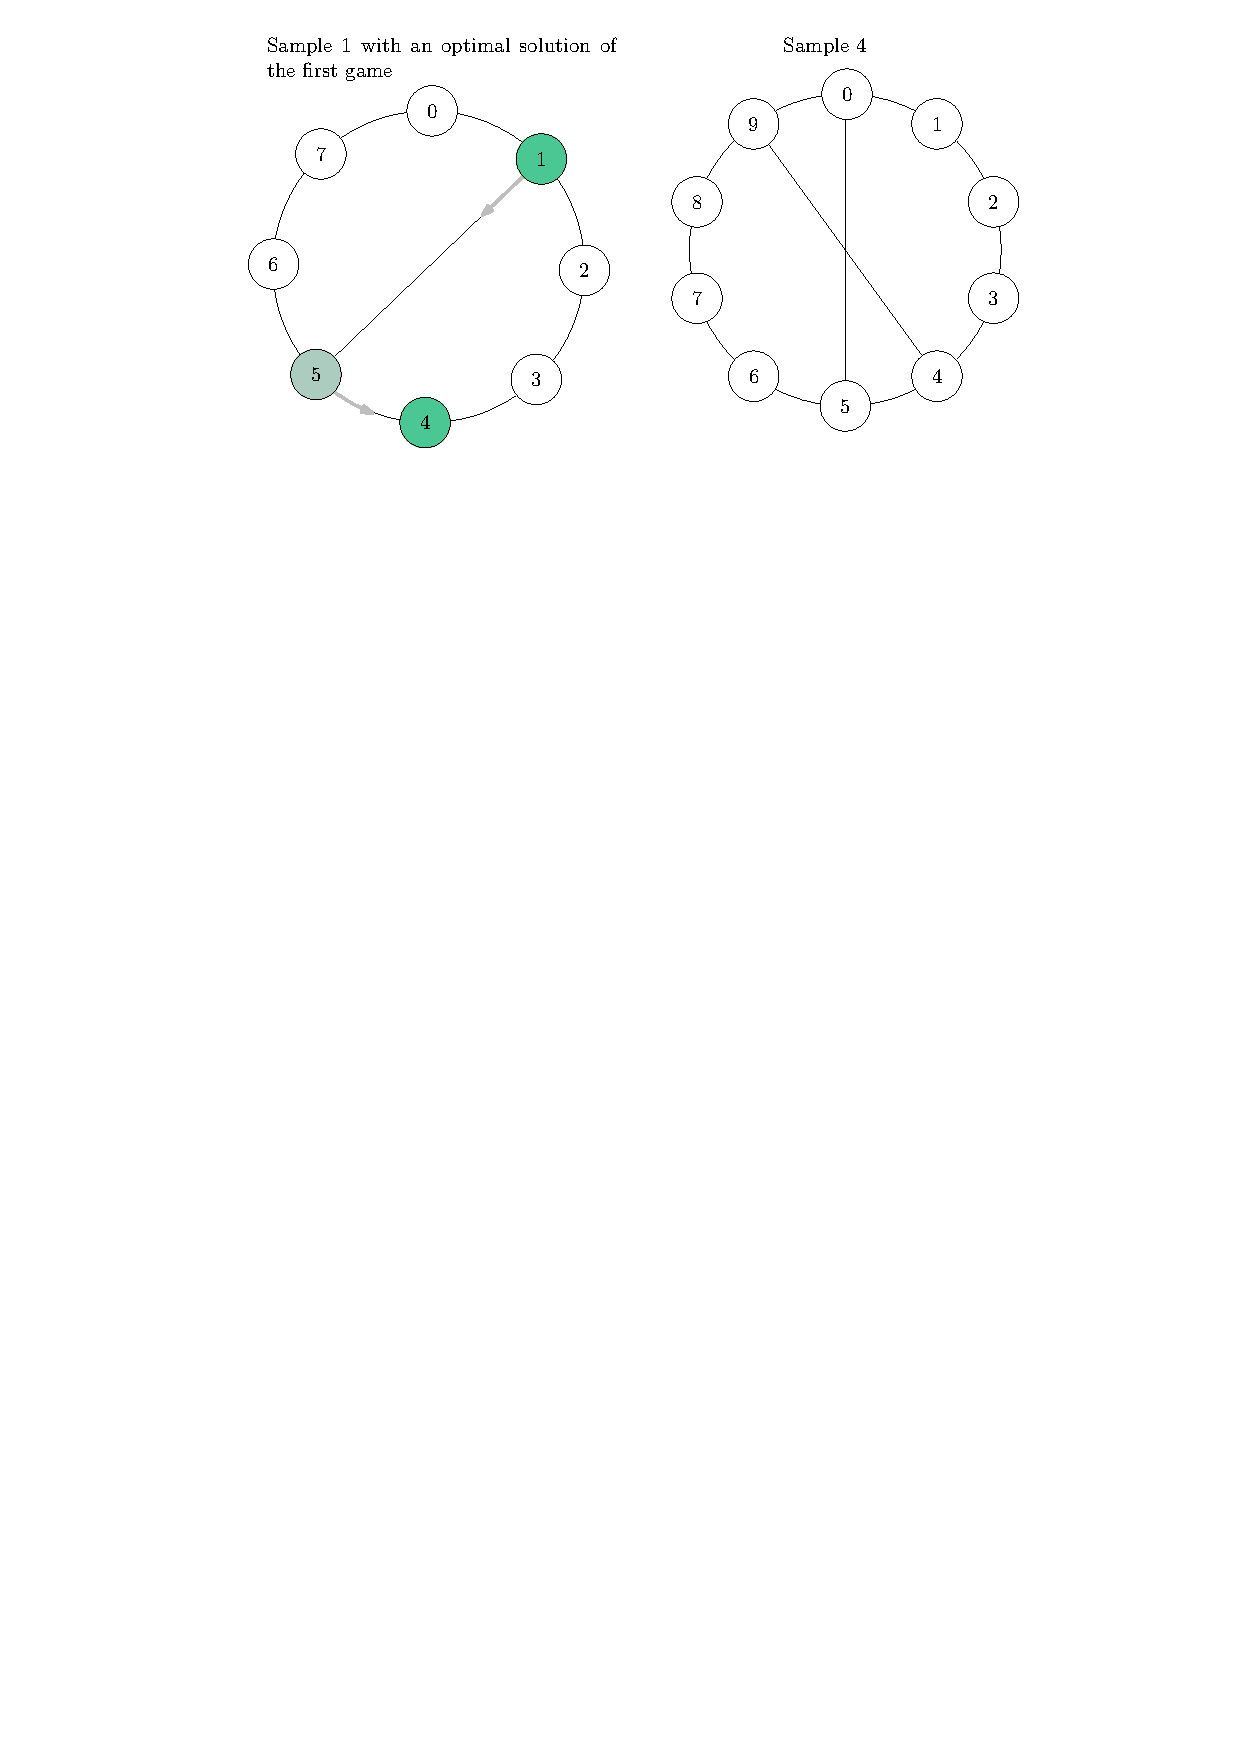
\includegraphics[width=0.7\textwidth]{sample1_4.pdf}
\end{center}

In the first game of the first sample, the ball is given to student $1$.
Student $1$ passes the ball to their best friend, student $5$.
The ball reaches student $4$ after student $5$ passes it to them, needing two passes in total.